% Chapter 2

\chapter{implementation theory and examples of designing mechanisms  }  % Main chapter title

\label{Chapter2} % For referencing the chapter elsewhere, use \ref{Chapter2} 

%----------------------------------------------------------------------------------------

% Define some commands to keep the formatting separated from the content 
%\newcommand{\keyword}[1]{\textbf{#1}}
%\newcommand{\tabhead}[1]{\textbf{#1}}
%\newcommand{\code}[1]{\texttt{#1}}
%\newcommand{\file}[1]{\texttt{\bfseries#1}}
%\newcommand{\option}[1]{\texttt{\itshape#1}}


\section{Introduction}
For dominant strategy implementation, we have mentioned the important
contributions of Hurwicz, Gibbard, Satterthwaite. In the first section
of this chapter, these results will be given in detail. These are
important impossibility theorems about which we can not design. Like
in physics, we know that we can not produce perpetual motion machine,
then we put our efforts on resource consuming machines which are
everywhere in use today. Likely, we should understand these proved
negative theorems well first, then we can begin our search on
mechanisms that can be designed and of some good qualities while
avoiding time waste on proved impossible mechanism design.


As we have mentioned in \ref{Chapter1}, the agents may have perfect
information regarding the economic environment $e$. In this case, Nash
Implementation is the solution concept most used. This we will deal
with in the next section.  If every agent $i$ knows his own $e_i$ and
knows the distribution of $e$, then this is the imperfect information
case which can be dealt with using Bayesian method.  These are mostly the
work of an old generation of  economic theorists but serve as good
reference points for comparison or provide basic
framework for some newer application. 

The economic environment $e$ in the following part and most economic literature is mostly the preference profile or utility profile, usually denoted $R$ or $u$.
\section{Important impossibility results}

\parencite{Gibbard1973 }
and \parencite{Satterthwaite1975} proved a very important theorem:If
the assignment results has at least 3 alterna-
tives, a social choice function which is strongly individually incentive compatible and
defined on a unrestricted domain is dictatorial.
\parencite{Gibbard1973} and \parencite{Satterthwaite1975} proposed a very important theorem for implementation theory. We will call it 
Gibbard Satterthwaite Impossibility theorem henceforth. It is stated like this.

\begin{thm}
If the outcome set $A$ has at least 3 alterna-
tives, a social choice rule which is strongly individually incentive compatible and
defined on a unrestricted preference domain is dictatorial.
\end{thm}

This impossibility result is very important. It lead the research to restricted preference domain, like in matching where the outcome is assumed to be ranked only by a player's self matched object. 

Pareto efficiency is often a basic requirement of economic
mechanisms. However, in \parencite{Hurwicz1972}
Hurwics  shows that  the Pareto efficiency and the truthful revelation is
fundamentally inconsistent even for the class of neoclassical economic
environments.
\begin{thm}
(Hurwicz Impossibility Theorem, 1972) For the neoclassical pri-
vate goods economies, there is no mechanism < M, h > that implements Pareto efficient
and individually rational allocations in dominant strategy. Consequently, any revelation
mechanism < M, h > that yields Pareto efficient and individually rational allocations is
not strongly individually incentive compatible. (Truth-telling about their preferences is not
Nash Equilibrium).
\end{thm}
The proof is adapted from Guoqiang Tian 2014.
\begin{proof}

By the Revelation Principle, we only need to show that any revelation mecha-
nism cannot implement Pareto efficient and individually rational allocations truthfully
in dominant equilibrium for a particular pure exchange economy.

Then, it is enough
to show that truth-telling is not a Nash equilibrium for any revelation mechanism that
yields Pareto efficient and individually rational allocations for a particular pure exchange
economy.

Consider a private goods economy with two agents and  two goods. The
endowments are 

$$w_1=(2,0), w_2=(0,2).$$

The utilities are

$$ u_i(x,y) = \begin{cases}
3x_i + y_i & \text{if $x_i\leq y_i$ } \\
x_i + 3y_i & \text{if $x_i>y_i$ }
\end{cases}$$

The above things form the economic environment $e$.

For the pure exchange economy, it has the following
allocation results set 
$$ A =\{( (x_1,y_1), (x_2,y_2))| x_1+x_2 = 2 \ and\ y_1+y_2=2 \}$$

Let $U$ be the set of all neoclassical utility functions, i.e. they are continuous and quasi-
concave, which agent i can report to the designer. Thus, the true utility function
$u_i \in U$.

Then, 
$$ h: U\times U \rightarrow A $$

Suppose that  the true utility function profile
$u_i$ were indeed a Nash Equilibrium, it would then  satisfy

\[ u_i(h(u_i, u_{-i})) \geq u_i(h(u'_i,u_{-i}))\]

\begin{tikzpicture}
\draw (0,0) rectangle (8,8);
\draw (0,0) -- (8,8);
\draw (8,0) -- (2,2)--(0,8);
\draw (8,0) -- (6,6)--(0,8);
\draw (0,8)--(8,0);
\node [below] at (2,2) {$a$};
\node [right] at (6,6) {$b$};
\node [right] at (4, 4) {$f$};
\node [below left] at (0,0) {$O_1$};
\node [above right] at (8,8) {$O_2$};


\end{tikzpicture}

Let us denote the individual rational allocations by $IR(e)$, the
Pareto efficient allocations by $P(e)$, the true report allocation
$d=h(u_i, u_{-i})$.

First thing to note is that the Pareto efficient allocation results is
all 
on the 45 degree line. For any other point, move on to the 45 degree
line along the shortest path( the path that is orthogonal to it) is a
Pareto improvement. $P(e)=O_1O_2$.  
Individual rational means that the final allocation must be at least
as good as the endowment, so $P(e) \cap IR(e) = \overline{ab}$ .

Suppose $d \in P(e) \cap IR(e)$, that is, $d \in \overline{ab}$.

If agent 1 misreports his utility function :

$$ u_1(x,y)=x_1 + y_1$$

Then, with the misreported $u_1$ and thus the misreported $e'$, the new set of individually rational and Pareto efficient allocations is given
by $P(e') \cap IR(e') = \overline{fb}$


If agent 2 misreports his utility function :

$$ u_2(x,y)=x_2 + y_2$$

Then, with the misreported $u_2$ and thus the misreported $e''$, the new set of individually rational and Pareto efficient allocations is given
by $P(e'') \cap IR(e'') = \overline{af}$

 If the $d$ is on $\overline{af}$, agent 1 will choose to
misreport a $u_1(x,y)=x_1 + ky_1$ where $0<k<1$. For any $d$ that is on $\overline{fb}$, agent 2 will choose to
misreport a $u_2(x,y)=x_2 + ky_2$ where $0<k<1$. 

Thus, no mechanism that yields Pareto efficient and individually rational allocations is
incentive compatible for both sides.


\end{proof}

\section{Nash implementation}
\parencite{Maskin1999} proposed a monotonicity concept that is later
called Maskin monotonicity, which is a necessary condition for Nash implementation. This condition along with no veto power
constitutes a simple set of  sufficient conditions 
for full Nash Implementation. 

Now, let us see the definintion of Maskin monotonicity.

\begin{definition}
A social choice rule $f: \mathscr{R} \rightarrow A$ satisfies Maskin
monotonicity provided that

$\forall a \in A, \forall R\ R' \in \mathscr{R},$, if $a \in f(R)$ and [
$\forall i \in \{1, \dots, n\} \forall b \in A  ,\  aR_i b \Rightarrow
aR'_i b$ ], then $ a \in f(R')$.
\end{definition}

Quoting \parencite{Maskin1999}, ``In words, monotonicity requires that if alternative $a$ is $f$ optimal with respect to some
profile of preferences and the profile is then altered so that, in each individual’s ordering,
$a$ does not fall below any alternative that it was not below before, then $a$ remains $f$ 
optimal with respect to the new profile.'' The $f$ optimal in the above quotation means that the alternative is chosen by the social choice rule $f$.

To illustrate the concept, \parencite{Maskin1999} provided some examples of
mechanisms satisfying Maskin Monotonicity. As a first example, he considered the Pareto optimal correspondence $f^{PO}$. 
If $a$ is (weakly) Pareto optimal with respect to $R$, then for all $b$,  $\forall i \ a R_i b$. Now if we replace $R$ by $R'$ such that, for all $i$, $a R_i b \Rightarrow  a R'_i b$, we conclude that
for all $b$, $\forall i \ a R'_i b$. Hence, $a$ is also (weakly) Pareto optimal with respect to $R'$,  establishing the monotonicity of $f^{PO}$.

The Condorcet correspondence $f^{CON}$ is also Maskin monotonic. If $a$ is a majority winner
for a strict profile (a profile consisting of strict orderings) $R$, then, for any other alternative
$b$, the number of individuals preferring $a$ to $b$ is no less than the number preferring $b$ to
$a$. Formally, 
$ |\{i|a R_i b\}| \geq |\{i|b R_i a\}| $ where the $|$s deliminating a set stands for the number of elements in the set.
Now if $R'$ is a profile such that, for all $i$, $a R_i b \Rightarrow a R'_i b$, then the left-hand side of the inequality cannot
fall when we replace $R$ by $R'$. Furthermore, if the right-hand side of the inequality rises, then a contradiction happens since for strict relation 
$R\ R'$ $|\{i|a R_i b\}| + |\{i|b R_i a\}|= |\{i|a R'_i b\}| + |\{i|b R'_i a\}|= n $. Therefore we conclude that the inequality continues to hold when $R'$ replaces $R$, and
so $a$ is still a majority winner with respect to the profile $R'$, establishing the monotonicity of $f^{CON}$.


The following  is an important theorem proposed by \parencite{Maskin1999}.


\begin{thm}
If $f: \mathscr{R} \rightarrow A$ is an SCR that is fully implementable in
Nash equilibrium, then it is Maskin monotonic.
\end{thm}
\begin{proof}
Suppose $f$ is fullly implementable in Nash equilibrium by the game form $h:
M_1\times \dots \times M_n \rightarrow A$.  Then for an arbitrary
profile $R \in \mathscr{R}$, and any $a \in f(R)$, because of full
implementation, there exists a Nash equilibrium $m$ of g with respect
to $R$ such that $h(m) = a$. Now consider a profile $R'$ that satisfy
the condition $\forall i \in \{1, \dots, n\} \forall b \in A  \  aR_i b \Rightarrow
aR'_i b$

If $m$ is not a Nash equilibrium with respect to $R'$,  then there
exists $i$ and $m'_i$ such that $h(m'_i, m_{-i}) P(R'_i) h(m) $. By
using the contrapositive of the above condition of $R'$, we get that there
exists $i$ and $m'_i$ such that $h(m'_i, m_{-i}) P(R_i) h(m) $, this
contradicts that $m$ is a Nash equilibrium. 
Therefore $m$ is a Nash equilibrium with respect to $R'$, by full
implementation, $h(m) \in f(R')$, i.e., $a \in f(R')$. Maskin
monotonicity of $f$ is proved.


\end{proof}

\parencite{Maskin1999} proposes a No Veto Power(NVP) concept, together with
Maskin monotonicity will be sufficient to guarantee full Nash
implementability. Here is its definition.

\begin{definition}
An social choice rule SCR $f:\mathscr{R} \rightarrow A$ satisfies NVP
if,
$\forall R \in \mathscr{R}$,$\forall a \in A$, and $\forall i \in
\{1,\dots, n\}$, 
($\forall j \not = i$ and $\forall b \in A$, $a R_j
b$) $\Rightarrow a \in f(R)$.
\end{definition}

Now the famous theorem of Maskin:
\begin{thm}
If $n\geq 3$ and $f: \mathscr{R}$ is a  n-person SCR satisfying Maskin
monotonicity and No Veto Power,  then it is implementable in Nash equilibrium.
\end{thm}

The proof of it is illustrative of how to prove implementability. It
is constructive as you can see. This proof method has been
in \parencite{Repullo90}.  \parencite{Maskin1999} adopted the same
approach. Here it is adapted. Only pure strategy is considered for implementability.

\begin{proof}

\end{proof}

Now we have a sufficient condition. However, it is not a necessary
condition. Two examples here.

\begin{example}
A constant social choice rule . A social choice rule SCR is called
a constant  social choice rule if  there is a $ C \subset A$ such that
$ \forall R \in \mathscr{R}, f(R) = C$. For a constant social choice
function, a Nash implementation mechanism can be given by letting  people
report their preference, and then choose the constant social choice
$C$ regardless of what they report.  Obviously, what ever the report
is, there is not profitable deviation. Therefore, every report profile
constitutes a Nash equilibrium whose result is the $C$, i.e., $h(m)=f(R)=C$.
\end{example}

\begin{example}
A  dictatorial  choice  rule. A social choice rule SCR is called a
dictatorial choice rule if $\exists i \in \{1,\dots,n\} $such that
$\forall R \in \mathscr{R}\  f(R) = top(R_i)$(here $top(R_i)$ means
the highest ranked $a \in A$ according to $R_i$). For a dictatorial
social choice function, a Nash implementation mechanism can be given by letting  people
report their preference, and then choose the dictator's top ranked
choice according to his or her reported preference regardless of what
others report. Obviously, what ever the others report, if the dictator
report his or her true preference, the result is a Nash equilibrium
profile. Therefore, every report profile
constitutes a Nash equilibrium whose result is the $top(R_i)$, i.e., $h(m)=f(R)=top(R_i)$.
\end{example}

The questions  are then:  what happens  in  the  grey  area  between
these  necessary and sufficient conditions of Nash implementation; and
what  happens  in the case  of two  agents? 


Actually, \parencite{Repullo90} has answered these questions.
\parencite{Danilov1992} provides another essentially monotone condition
that is  necessary and sufficient. \parencite{Yamato1992} extended the
\parencite{Danilov1992}  conditions for Nash implementation to weak
preferences over an arbitrary set of alternatives. Anyway,
these necessary  and sufficient  condition was not easy to identify,
and  \parencite{Maskin1999} proposed the easier to identify
sufficient condition and a separate necessary condition that are
well-known as Maskin monotonicity(Actually, the paper as a working paper is widely known since 1977 and all the later papers
 had been written under the influence of it).   \parencite{Maskin1999} has been
widely known since 1977 as working paper, and all these necessary and
sufficient condition has been greatly influenced by Maskin's work. In this retrospective
chapter, we would like
to have a look at these conditions. 

\subsection{Condition $\mu$}

First, let us take a look at the necessary and sufficient condition
in \parencite{Repullo90} which is the most general form of condition
. It is called condition $\mu$ which contains three parts.
\begin{definition}
  Condition $\mu$: There is a set $B \subset A$, and $\forall i \in I,
  R\in\mathscr{R}, a \in f(R)$, there is a set $C_{i}(a, R) \subset
  B$, with $a \in M_{i}(C_{i}(a,R),R)$ such that $\forall R^* \in
  \mathscr{R}$, the following (i), (ii) and (iii) are satisfied.

(i) if $a \in \cap_{i \in I} M_i(C_i(a, R),R^*)$, then $ a \in f(R^*)$.

(ii)if $c \in M_i(C_i(a, R), R^*) \cap [ \cap_{j \not = i} M_j(B, R^*)]$, then $c \in f(R^*)$.

(iii)if $d \in \cap_{i\in I} M_i(B, R^*)$, then $d \in f(R*)$. 

\end{definition}
In the above definition, $I= \{1,\dots,n\}$, and the $M_{i}$ has the following meaning. For
any $i \in I, R \in \mathscr{R}, C \subset A$, $M_{i}(C, R)$ denote
the set  of maximal  elements  in $C$ for  agent  $i$  under  preference $R_{i}$.

Now, the theorem in \parencite{Repullo90} is cited here.

\begin{thm}
\label{mu}
  Suppose there are three or more agents. Then a choice rule $f$ is Nash implementable if and only if it satisfies Condition $\mu$.
\end{thm}

\begin{proof}
Necessity.  There must be a range for the Nash implementing mechanism
$\Gamma = \langle S, g\rangle$. Let it be the $B$ in condition $\mu$.

\[ B\equiv \{a \in A|a=g(s)\ for\ some\ s \in S\}\]

 According to full Nash implementation, $\forall  R\in\mathscr{R}, a \in f(R)$, there is a Nash equilibrium profile $s$
 implementing the $a$, denote it by $s(a, R)$.  $\forall i \in I$,  we choose 
\[C_i(a,R)\equiv \{ c \in A | c = g(s'_i,s_{-i}(a,R))\  for\  some\  s'_i \in
  S_i\}\]
After finding the $B$ and $C_i$,  $\forall R^* \in \mathscr{R}$, condition $\mu$ (i)(ii)(iii)  are
directly implied by the full Nash implementation.

if $a \in \cap_{i \in I} M_i(C_i(a, R),R^*)$, then $s(a,R)$ is a Nash
equilibrium of the mechanism under $R^*$.  Since the mechanism fully
implement the social choice rule $f$, $a \in f(R^*)$.

if $c \in M_i(C_i(a, R), R^*) \cap [ \cap_{j \not = i} M_j(B, R^*)]$,
then $c = g(s'_i,s_{-i}(a,R))$ and is the best outcome among outcomes with the form
  $g(\hat{s_i},s_{-i}(a,R))\  where \  \hat{s_i} \in
  S_i$  under $R^*$, and $c$ is the best outcome for all $j \not = i$ in $B$ under
  $R^*$.  Therefore $(s'_i,s_{-i}(a,R))$  is a Nash
equilibrium of the mechanism under $R^*$.  Since the mechanism fully
implement the social choice rule $f$, $c \in f(R^*)$.

if $d \in \cap_{i\in I} M_i(B, R^*)$, then $d$ is the best outcome for
all $i \in I$ under $R^*$ and therefore the strategy profile $s(d,R*)$
producing $d$ is a Nash equilbrium of the mechanism under $R^*$. 
Since the mechanism fully
implement the social choice rule $f$, $d \in f(R^*)$. Thus, necessity
is  proved.

Sufficiency. For any  $f$ satisfying the condition $\mu$, it  is
enough to construct a mechanism $\Gamma$ which Nash
implements the social choice rule $f$  fully. The construction method of such
a mechanism is adapted
from the appendix of \parencite{Repullo90}. 

For each agent $i \in I$ , the message or strategy space is 
\[ S_i \equiv \mathscr{R} \times A \times Z^+ \]
and the outcome function $g: S \rightarrow A$ is defined as follows.

Case 1. If $\forall i \in I, s_i =  (R, a, n)$ such that $R \in
\mathscr{R}, a \in A, n \in Z^+$, then $g(s)=a$.

Case 2. If $\exists i \in I, \forall j \not = i \ s_j=(R, a, n) \  and
\ s_i = (R', a', n')$ where $ (R, a, n)  \not = (R', a', n')$, then 
$$g(s)= \begin{cases} 
 a'  & \text{if $a' \in C_i(a, R)$}\\ 
 a  & \text{otherwise} \end{cases}$$

Case 3. For all the other situations, $g(s) = a_i$, where $a_i$ is the agent with the largest
reported $n$'s choice of  $a$ (ties are broken by random selection).

Thus, the mechanism $\Gamma$ is fully defined.
We need to prove $\forall R in \mathscr{R} f(R) = NE(\Gamma, R)$. For
any $R \in \mathscr{R}$, the following two facts are showed to
complete the proof.

$f(R) \subset NE(\Gamma, R)$. $\forall a \in f(R)$, we consider the
strategy profile $s$ satisfying that $\forall i \in I, s_i = (R, a,
1)$. It is a Nash equilibrium, because  if one deviates, Case 2
stipulates that other than $a$ only an $a' \in C_i(a,R)$ can be chosen
which is worse than $a$ according to condition $\mu$($a \in
M_{i}(C_{i}(a,R),R)$ ).

$NE(\Gamma, R) \subset f(R)$.  There are three equilibrium
cases. 

Case1: $\forall i \in I, s_i =  (R', a, n)$ , then $g(s)= a \in
\cap_{i \in I}M_i(C_i(a,R'), R)$ because deviation can lead to any
element in $C_i(a,R')$ and Nash equilibrium should guarantee no
profitable deviation. By condition $\mu$ (i), $g(s) \in f(R)$.

Case2: $\exists i \in I, \forall j \not = i \ s_j=(R', a, n) \  and
\ s_i = (R'', a', n')$ where $ (R', a, n)  \not = (R'', a', n')$, then
$$g(s)= \begin{cases} 
 a'  & \text{if $a' \in C_i(a, R')$}\\ 
 a  & \text{otherwise} \end{cases} $$

and $g(s) \in  \in M_i(C_i(a, R'), R) \cap [ \cap_{j \not = i} M_j(B,
R)]$ because $i$'s deviation can lead to any element in $C_i(a, R')$
while $\forall j \not = i$  $j$'s deviation can lead to any element in $B$ by
anouncing a big enough $n$. By condition $\mu$ (ii), $g(s) \in f(R)$.


Case3: For all the other situations other than the previous two cases,
anyone can pronouce a big enough $n$ to get any  element in $B$. Nash
equilibrium means that the chosen $g(s)=a \in \cap_{i\in I} M_i(B,
R)$. By condition $\mu$ (iii), $g(s) \in f(R)$.








\end{proof}

%For the proof, see the original paper. 

A explanation of the condition $\mu$ is needed here. It is not as complex as one may feel at a quick glance. In fact, 
condition $\mu$ (i) is an equivalent of Maskin monotonicity.  To see
this, let $C_i(a,R)= L_i(a,R)$, then Maskin's monotonicity
$\Rightarrow$ condition $\mu$ (i). The other direction,  condition
$\mu$ (i) $\Rightarrow$ Maskin's monotonicity , is shown as follows.
Choose any  $R, R' \in \mathscr{R}$ and $a \in f(R)$ such that $L_i(a, R)
\subset L_i(a, R')$ for all $i \in I$. From  Condition $\mu$ we know
that  for  each $i \in I$ and $R \in \mathscr{R}$ there  exists  a set
$C_i(a, R)$ such  that  $a \in  M_i(Ci(a,  R),  R)$  implying  that
$C_i(a, R) \subset  L_i(a,R)$.   Hence $C_i(a, R) \subset  L_i(a,R')$,
which is equivalent to $a \in \cap_{i \in I}M_i(C_i(a,R),
R')$. Therefore by condition $\mu$ (i) we conclude that $a \in
f(R')$.  $f$ is thus shown to be monotonic.

Condition $\mu$ (ii) (iii) are implied by No Veto Power. Let $B=A$, and 
we can see this easily.

To see the usage of such a necessary and sufficient condition, a proof
of a proposition is provided.

First,  introduce a concept called neutral social choice rule.
\begin{definition}   
Formally,  a choice rule  f  is  said  to  be neutral  if  for  all  permutations  $\pi:  A \rightarrow A$  and  $R \in \mathscr{R}$
  we have an $R^\pi \in \mathscr{R}$ such that $f(R^\pi) = \pi \circ f(R) $  and  $\forall i \in I: a R^\pi_i b \Longleftrightarrow \pi^{-1}(a) R_i \pi^{-1}(b)$.  
  \end{definition}

That is, a neutral social choice function does not care about what the
allocation really is, it only cares about what the agents has ranked
these allocations and then decides. Apparently, a constant social
choice rule  is not neutral. However, a dictatorial social choice
rule is neutral as you can check according to the definition.


\begin{prop}
  Suppose there are three or more agents. Then a choice rule f is
Nash implementable if it is monotonic and neutral.
  
\end{prop}

\begin{proof}

Now we will prove it by condition $\mu$ and theorem \ref{mu}.

Monotonicity is equivalent to condition $\mu$ (i). Now we need to show
monotonicity and neutral imply
condition $\mu$ (ii)(iii).

For the implication of condition $\mu$ (ii). $\forall R, R' \in
\mathscr{R}, a \in f(R), i \in I$, if $c \in M_i(C_i(a, R), R') \cap [ \cap_{j
  \not = i} M_j(B, R')]$, we need to show $c \in f(R')$. Choose $R''
\in \mathscr{R}$ such that it is the same as $R$ except that outcomes
$a$ and $c$ are switched. By neutrality, $a \in f(R) \Rightarrow c \in
f(R'')$. By monotonicity, $c \in f(R'')  \Rightarrow c \in f(R')$ as
required.

For the implication of condition $\mu$ (iii). $\forall R' \in
\mathscr{R}$, if $ d \in \cap_{i \in I}M_i(B, R')$, we need to show $d
\in f(R')$. Choose $h \in f(R')$. If $h = d$, then the proof is done. 
If $h \not = d$, choose $\hat{R}
\in \mathscr{R}$ such that it is the same as $R'$ except that outcomes
$d$ and $h$ are switched. By neutrality, $h \in f(R') \Rightarrow d
\in f(\hat{R})$. By monotonicity, $d \in f(\hat{R}) \Rightarrow d \in
f(R')$ as required.
\end{proof}

%Formally,  a choice rule  f  is  said  to  be neutral  if  for  all  permutations  π :  A → A  and  θ ∈ Θ  we have θπ ∈ Θ and π·  f(θ)  %=f(θπ)-where  the  profile θπ is  such that  for  all  i ∈ I: aRi(θπ)b if and  only  if π -1(a)Ri(θ)π -1(b).  

%Condition $\mu$: There  is  a  set  B ⊂A,  and  for each  i ∈ I, θ ∈ Θ, and a∈f(θ), there  is  a set Ci(a,  θ) ⊂B, with 
 %    a∈Mi(Ci(a,  θ), θ )  such  that  for  all θ*∈ Θ,  the following (i),  (ii) and  (iii)  are satisfied. 
 % (i)if a∈∩ i ∈ IMi(Ci(a,  θ), θ* ) , then a∈f(θ*).
  %(ii)if c∈Mi(Ci(a,  θ), θ* ) ∩(∩j≠iMj(B, θ* )), then c∈f(θ*).
  %(iii)if d∈∩ i ∈ IMi(B, θ* ), then d∈f(θ*).
%For  any i∈I ,  θ∈Θ, and  C⊂A,  let  Mi (C, θ)  denote the set
%of maximal  elements  in C for  agent  i  under  θ.

\subsection{Essentially monotonic}
\parencite{Danilov1992}  proposed an essentially monotone concept
and \parencite{Yamato1992} extended its application conditions and
called it strongly monotonic. We will call it essentially  monotonic in this
paper. 

Some definitions are needed. First, the notion of essential element
for a participant in a particular set of outcomes.

\begin{definition}
For any $i \in I$ and $X \subset A$, an alternative $x \in X$ is
essential for $i$ in set $X$ if $\exists R \in \mathscr{R}$ such that
$x \in f(R)$ and $ L_i(x, R) \subset X$.
\end{definition}

The set of all essential elements for $i$ in $X$ under a social choice
rule $f$ is denoted as $Ess_i(X, f)$.

We can now define the notion of essential monotonicity.

\begin{definition}
A social choice rule $f$ is essentially monotonic if $\forall R, R' \in
\mathscr{R}, a \in f(R)$,  $Ess_i(L_i(a, R), f)
\subset L_i(a, R') for all  i \in I$ implies $a \in f(R')$. 
\end{definition}

A useful rewrite of this essentially monotonic condition is provided
in \parencite{Yamato1992}. That is, a social choice rule satisfies essential
monotonicity if :  $\forall R, R' \in \mathscr{R}, a \in f(R), a \not
\in f(R')$,  there exists $i \in I, b \in A$ such that (i) $a R_i b$
and $b P_i a$; (ii) $\exists \hat{R} \in \mathscr{R}$, $b \in
f(\hat{R})$ and $L_i(b, \hat{R}) \in L_i(b, R)$.
This rewrite has done a contrapositive to the definition and
insert in the definition of essential elements $Ess$. 

\begin{remark}
Some properties of essential elements and essential monotonicity are
listed here. 

For any $ B \subset C \subset A$,  $Ess_i(B,f) \subset Ess_i(C,f)
\subset Ess_i(C,f) \subset Ess_i(A,f) = Im(f)$. Essential monotonicity
implies Maskin monotonicity, because $Ess_i(L_i(a, R), f) \subset L_i(a,R)$.
\end{remark}


\parencite{Yamato1992} proposed a requirement of Condition $D$ on the preference
domain $\mathscr{R}$.

\begin{definition}
The preference domain $\mathscr{R}$ satisfies Condition $D$ if
$\forall a \in A, r \in R, i \in I, b \in L_i(a, R)$, there exists $R'
\in \mathscr{R}$ such that $L_i(a,R) = L_i(b, R')$ and $\forall j \not
= i  L_j(b,R')=A$
\end{definition}

Condition $D$ can be thought as a requirement that the preference
domain $\mathscr{R}$ should contain sufficiently many
preferences. For example, unrestricted domain therefore easily
satisfies condition $D$.

The following necessity theorem of Nash implementation is
from \parencite{Yamato1992}.

\begin{thm}
If the preference domain $\mathscr{R}$ satisfies Condition $D$, and
a social choice rule $f :\mathscr{R} \rightarrow A$ is fully Nash
implementable, then $f$ is essentially monotonic.

\end{thm}

\begin{proof}
Suppose mechanism $\Gamma=(S,g)$ Nash implements a  social choice rule
$f$, $R, R' \in \mathscr{R}$. Due to full implementation, $f(R)=
g(NE(R))$ and $f(R')= g(NE(R'))$. We then use  the contrapositive rewrite of
the essential monotonicity definition mentioned above to show that $f$
is essentially monotonic. For any $a \in f(R)$ and $a \not \in f(R')$,
there is a $ s \in NE(R)$ such that $a =g(s)$ ; there is a $i \in I, b
= g(s'_i, s_{-i})$ such that  $ b P'_i a$. Obviously  $b \in L_i(a,
R)$ by Nash equilibrium concept, so the (i) of the rewrite
of essential monotonicity is fulfilled. From condition $D$, $\exists
\tilde{R} \in \mathscr{R}$ such that $L_i(b, \tilde{R})=L_i(a,R)$
and $\forall j \not = i, L_j(b, \tilde{R})=A$. Since $g(S_i, s_{-i})
\subset L_i(a,R) $ and $\forall j\not = i, g(S_j, s_{-j}) \subset A$, therefore $g(S_i, s_{-i})
\subset L_i(b, \tilde{R}) $ and $\forall j \not = i, g(S_j, s_{-j})
\subset L_j(b, \tilde{R})$. $b \in NE(\tilde{R}) = f(\tilde{R})$.
\end{proof}

The sufficiency theorem of Nash implementation for more than 3
participants are proposed and proved in both \parencite{Danilov1992}
and \parencite{Yamato1992}. The following is the theorem.

\begin{thm}
If there are more than 3 participants, then an essentially monotonic
social choice rule  is fully Nash implementable.
\end{thm}

%\begin{proof}
\begin{comment}
The method is still by construction. For a essentially monotonic
social choice rule $f$. We construct the following mechanism.

The construction method of such
a mechanism is adapted
from the appendix of \parencite{Repullo90}. 

For each agent $i \in I$ , the message or strategy space is 
\[ S_i \equiv \mathscr{R} \times A \times Z^+ \]
and the outcome function $g: S \rightarrow A$ is defined as follows.

Case 1. If $\forall i \in I, s_i =  (R, a, n)$ such that $R \in
\mathscr{R}, a \in A, n \in Z^+$, then $g(s)=a$.

Case 2. If $\exists i \in I, \forall j \not = i \ s_j=(R, a, n) \  and
\ s_i = (R', a', n')$ where $ (R, a, n)  \not = (R', a', n')$, then 
$$g(s)= \begin{cases} 
 a'  & \text{if $a' \in C_i(a, R)$}\\ 
 a  & \text{otherwise} \end{cases}$$

Case 3. For all the other situations, $g(s) = a_i$, where $a_i$ is the agent with the largest
reported $n$'s choice of  $a$ (ties are broken by random selection).

Thus, the mechanism $\Gamma$ is fully defined.
We need to prove $\forall R in \mathscr{R} f(R) = NE(\Gamma, R)$. For
any $R \in \mathscr{R}$, the following two facts are showed to
complete the proof.

$f(R) \subset NE(\Gamma, R)$. $\forall a \in f(R)$, we consider the
strategy profile $s$ satisfying that $\forall i \in I, s_i = (R, a,
1)$. It is a Nash equilibrium, because  if one deviates, Case 2
stipulates that other than $a$ only an $a' \in C_i(a,R)$ can be chosen
which is worse than $a$ according to condition $\mu$($a \in
M_{i}(C_{i}(a,R),R)$ ).

$NE(\Gamma, R) \subset f(R)$.  There are three equilibrium
cases. 

Case1: $\forall i \in I, s_i =  (R', a, n)$ , then $g(s)= a \in
\cap_{i \in I}M_i(C_i(a,R'), R)$ because deviation can lead to any
element in $C_i(a,R')$ and Nash equilibrium should guarantee no
profitable deviation. By condition $\mu$ (i), $g(s) \in f(R)$.

Case2: $\exists i \in I, \forall j \not = i \ s_j=(R', a, n) \  and
\ s_i = (R'', a', n')$ where $ (R', a, n)  \not = (R'', a', n')$, then
$$g(s)= \begin{cases} 
 a'  & \text{if $a' \in C_i(a, R')$}\\ 
 a  & \text{otherwise} \end{cases} $$

and $g(s) \in  \in M_i(C_i(a, R'), R) \cap [ \cap_{j \not = i} M_j(B,
R)]$ because $i$'s deviation can lead to any element in $C_i(a, R')$
while $\forall j \not = i$  $j$'s deviation can lead to any element in $B$ by
anouncing a big enough $n$. By condition $\mu$ (ii), $g(s) \in f(R)$.


Case3: For all the other situations other than the previous two cases,
anyone can pronouce a big enough $n$ to get any  element in $B$. Nash
equilibrium means that the chosen $g(s)=a \in \cap_{i\in I} M_i(B,
R)$. By condition $\mu$ (iii), $g(s) \in f(R)$.
\end{comment}
%\end{proof}

An application of this essential monotonicity concept is provided
in \parencite{SonmezJet1996}.  There they proved that 
\section{Some examples of  mechanisms}

The previous results are formal and  mathematical. The following will give some examples of mechanism design.

\subsection{Assets Inheritance problem}
\begin{example}
An old man has lots of  houses and three sons. When he is about to die, he
want to give the houses to his sons, but he is not familiar with the
market prices for these houses. He does not want to make the sons
share any house, so he would like to  give every  house as a whole to some son. All  sons know the prices of these
houses well. all  sons like more values from the
inherited houses. How can he achieve his goal of dividing the houses as
fairly as possible, but if it can not be perfect fair, he prefers to
give his younger sons more. 

The fairness here means that to make the least valued group of assets as close to the average as possible.

\end{example} 

For the example situation, can a mechanism be designed so that the old
man's goal be implemented? The best mechanism should be let the oldest son to devide the assets or houses into 3 groups, then let the youngest son chooses first, and the middle son chooses second, and the oldest
son gets what is left. This is the simple but effective way of implementing the choice rule. Another form of the mechanism that is basically the same thing is that let the three sons report the values of the assets
. and then devide the assets as fairly as possible according to what the oldest son has reported. The social planner picks the most valuable group of assets according to the youngest son's report and 
give it to him, 
then picks the more valuable group from the remaining assets according to the middle son's value report, and finally gives the last group of goods to  the oldest son.

\subsection{An example of Auction Design}
In the last part of the chapter, we would like to design a mechanism for selling goods with  uncertain values.  Here a distribution assumption is used. Auctions are one of the most successful areas where the development of economics
theory and practice help each other. I will try to investigate this area from
a mechanism design perspective in this section. The material is put here as an example of what can be implemented for some special market. 

Here we focus on revenue maximization for the seller of an indivisible experience
good under a situation in which buyers are all ex-ante identical. The only information they all have is an identical
value distribution of the experience good. In our
setting, the seller can freely give any buyer access to get his true private value, which process we call experiencing the good. If the seller is
unable to charge experience fee, she may maximize her revenue by excluding just one buyer from experiencing, which is in conflict with the social efficiency. If
the seller is able to charge experience fee, she will maximize her revenue through setting
the price at a level such that every potential buyer will buy the experience, 
resulting in the maximal trading surplus which is fully extracted by the seller.

Of course, the equilibrium of implementation in such a mechanism is ex ante,  the following chapter will be concerned with ex post implementation.

Now the details are as follows. A seller(she) has a single indivisible good, and wants to sell the good to a group of $N$ buyers indexed by $i=1, 2, . . . , N$(buyers and
bidders are used interchangeably in this paper, and are assumed to be
male). All parties are risk neutral. 
 The value of retaining the good to the seller
is publicly known as $\underline{v}(\geq 0)$ in this paper. Bidder i's valuation of the object
is $v_{i}$, and $v_{i}$ has independent identical distribution $F(x)$ with support $[\underline{v}, \overline{v}]$, 
where $\overline{v}>\underline{v}$, and $\overline{v}=+\infty$ is allowed. 
In the beginning, no one can directly observe the $v_{i}$. Only the distribution is common knowledge among all the parties. However, if the seller gives a chance of experiencing the good to a buyer, the buyer can learn of his $v_{i}$ after experiencing. 
 

The seller designs a sales mechanism to sell the
good. The sales mechanism consists of two stages, the experience stage, and the auction stage. 
After the experience stage, the seller will allow those who
have experienced the good to
participate the auction. By Revenue Equivalence Principle, we analyze the case that the seller chooses the second-price
sealed-bid auction in the auction stage without loss of generality. In the auction stage, if no bidder bids a value exceeding a reserve price
, then the good is sold to the unexperienced buyer at the
price $\mu$(the expectation of v) when there is an unexperienced buyer. Here we assume that the buyer will choose to buy the good if he is indifferent between buying and not buying the good. 
The timeline is shown in the Figure 1. 
\begin{figure}
\begin{center}
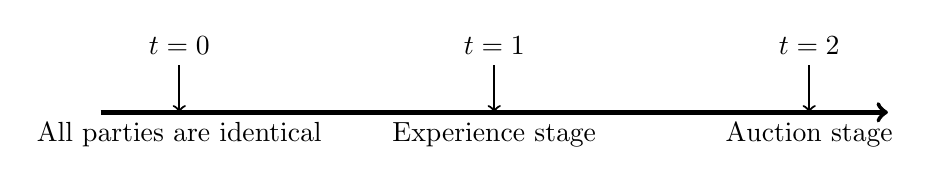
\begin{tikzpicture}
 \draw[->, ultra thick] (5, 0) -- (15, 0);
 \draw[->, thick](6, 0. 6)node[above]{$t = 0$} -> (6, 0)node[below]{All parties are identical } ;
 \draw[->, thick](10, 0. 6)node[above]{$t = 1$} -> (10, 0)node[below]{Experience stage};
 \draw[->, thick](14, 0. 6)node[above]{$t = 2$} -> (14, 0)node[below]{Auction stage} ;
 \end{tikzpicture}
\end{center}
 \caption{Timing of experience good auction }
\end{figure}

\subsubsection{Setting Reserve price to extract trade surplus}
In the situation that the seller cannot charge fee for experiencing the good, 
the seller will set a reserve price in the auction stage to maximize the
revenue in a second-price sealed-bid auction. 
\begin{lemma}\label{lem}
 The hazard rate function associated with the distribution F is
defined as $\lambda(x) = f(x) / (1 - F(x))$. The optimal reserve price $r$ satisfies $r - 1/\lambda(r)= v^*$. The $v^*$ denotes the seller's reserve revenue/valuation. 
\end{lemma}
\begin{proof}
Let $R(r, m)$ denote the revenue of the seller when the reserve price is $r$ and the number of buyers experiencing the good is $m$. 

Obviously, $r$ should be higher than $v^*$ to have an effect of enhancing the price. 
Then the expected value of seller revenue can be calculated as the sum of three parts, the revenue from the auction when the second highest bid is above the reserve price $r$, the revenue from the auction when the highest bid is above the reserve price but the second highest price is below the reserve price $r$, and the reserve revenue/valuation$v^*$ when the highest bid is below the reserve price $r$. 
\begin{equation}\label{equ}
R(r , m) =\int_{r}^{\overline{v}}x\mathrm{d}G_{(2)}^{m}(x) + rmF^{m-1}(r)[1 - F(r)] + v^* F^{m}(r)
\end{equation}
where $G_{(2)}^{m}(x) = F^{m}(x) + mF^{m-1}(x)[1 - F(x)]$. 


Differentiating this with respect to $r$ and simplify, we obtain
$$-rmF^{m-1}f(r)+mF^{m-1}(r)(1-F(r))+v^* mF^{m-1}(r)f(r)$$

The first order condition is 
$$r^* - \frac{1 - F(r^*)}{f(r^*)} = v^*$$
\end{proof}
\begin{remark}
 Under regularity conditions, the first order condition is also sufficient for optimality. 
\end{remark}
 If the seller gives a buyer the chance to experience the good, no buyer will refuse since experiencing the good means some chance
of gain. Thus the number of buyers who can experience the good is at her control. Intuitively, she 
wants to obtain a high revenue from the auction by letting more buyers to experience as long as there is still an unexperienced buyer, for the seller can sell the good to him
at price $\mu$ when no bidder bids over the
reserve price. This is summarized in the following proposition. 
\begin{prop}
 As the number m of buyers experiencing the good increases, the expected value of seller revenue increases as long as $m\leq n-1$. 
\end{prop}
\begin{proof}
When the reserve revenue $v^*$ is obtained by selling the good to a 
unexperienced buyer, $v^*=\mu$. Then by equation~\ref{equ} in the proof of Lemma~\ref{lem}, 
\begin{equation}
R(r, m) = \int_{r}^{\overline{v}}x\mathrm{d}G_{(2)}^{m}(x) +
rF^{m-1}(r)[1 - F(r)] + \mu F^{m}(r)
\end{equation}
where $G_{(2)}^{m}(x) = F^{m}(x) + mF^{m-1}(x)[1 - F(x)]$. 

When $m\leq N-1$, the best reserve price is $r=r^*$ which is the solution to $r^*-1/\lambda(r^*)=\mu$. The revenue is $R(r^*, m)$. 
 By the first order stochastic dominance, it is straightforward to show $R(r^*, m) > R(r^*, m')$ for any $N-1\geq m>m'$. 
\end{proof}
However, letting $N$ potential buyers to all experience the good may
not be better than just letting $N-1$ buyers to experience. Because the former may let go the
safe option of selling the good at $\mu$. Indeed, it depends on the
distribution F(x). A careful research of us has led to the following conclusion. 
\begin{thm}
 The seller does not always want all buyers to experience the good under the setting here. 
 \end{thm}
 \begin{proof}
 When every buyer has experienced the good, then by lemma~\ref{lem}, 
 the reserve price should now be set to $\hat{r}$, which is the solution to $\hat{r}-1/\lambda(\hat{r})=\underline{v}$, since the reserve
valuation is $\underline{v}$ and the revenue 
is $R(\hat{r}, N)$ using equation~\ref{equ}. 
Generally speaking, 
 $R(\hat{r}, N)<R(r^*, N-1)$ for many distributions and the potential buyers' number N. 
 \end{proof}
Figure 2 shows the values of $R(r^*, N-1)-R(\hat{r}, N)$ for different
values of parameters in Beta distribution(with the horizontal axis denoting N). 
\begin{figure}
\centering
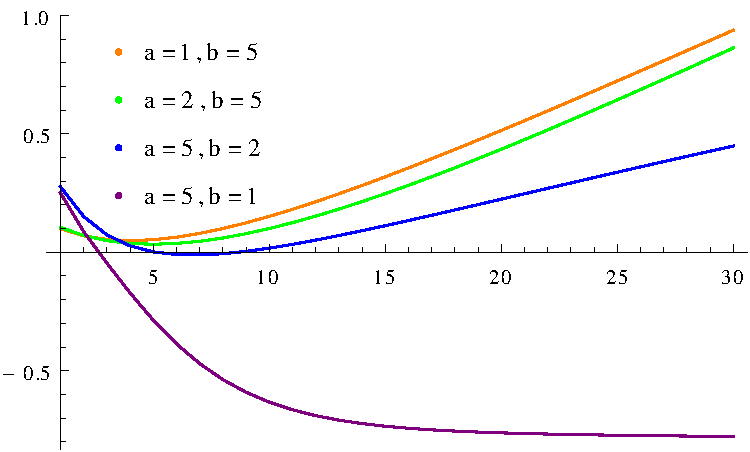
\includegraphics[width = 11cm]{betaGraph.pdf}
\caption{Difference in revenue: $R(r^*, N-1)-R(\hat{r}, N)$} \label{fig:graph}
\end{figure}

\begin{remark}
 Specially for the uniform distribution, we have, when $N\leq 7$, $R(\hat{r}, N)<R(r^*, N-1)$. 
\end{remark}

\subsubsection{Charging Experience fee to extract trade surplus}
 We then consider the case where the seller can charge experience fee. For the seller, at the experience-stage, how to optimally set price of exprience? 
If a certain number of buyers are permitted to experience the good, each of those buyers is supposed to get a nonnegative ex ante expected payoff from participating the
subsequent second-price auction. Suppose that buyers will buy the experience when they are indifferent between remaining
uninformed and buying the experience to be informed. 
 Then the seller should set the price equal to a buyer's ex ante expected payoff of participating the auction to extract all the expected trade surplus. Intuitively, the ex ante expected payoff of experiencing buyers depends on the number of auction partipants. 
%First, we set the prespecified price as $\mu$ for the auction. Then the expected result of the auction can be calculated. \end{comment}



Next, we will offer the formula for the experience fee in the following lemma. 
\begin{lemma}
 The experience fee $P(m)$ can be formulated as 
\begin{equation}
 P(m) = \begin{cases}\int_{\mu}^{\overline{v}}\int_{\mu}^vF^{m-1}(t)\mathrm{d}tf(v) \mathrm{d} v, &\textrm{if}\quad m \leq N-1\\
\int_{\underline{v}}^{\overline{v}}\int_{\underline{v}}^v F^{N-1}(t)\mathrm{d}tf(v) \mathrm{d} v, &\textrm{if}\quad m = N
\end{cases}
\end{equation}


\end{lemma}
\begin{proof}
 When there are $m(\leq n-1)$ buyers knowing one's own value information, the value of the information is
\begin{align*}
P(m)&= \int_{\mu}^{\overline{v}}(\int_{\mu}^v (v-t)\mathrm{d}F^{m-1}(t)+(v-\mu)F^{m-1}(\mu))f(v)\mathrm{d}v \\
&= \int_{\mu}^{\overline{v}}\int_{\mu}^vF^{m-1}(t)\mathrm{d}tf(v)\mathrm{d}v
\end{align*}

$P(N)$ can be formulated as, 
 \begin{align*}
P(N) &= \int_{\underline{v}}^{\overline{v}}\int_{\underline{v}}^v(v-t)\mathrm{d}F^{N-1}(t)\mathrm{d}tf(v)\mathrm{d}v \\
 &= \int_{\underline{v}}^{\overline{v}}\int_{\underline{v}}^v F^{N-1}(t)\mathrm{d}tf(v)\mathrm{d}v
\end{align*}
\end{proof}

\begin{lemma}
As the number of buyers knowing one's own value information increases, the expected value of knowing one's own value information decreases. 
\end{lemma}
Notice that for many distributions and potential buyers' number n, $P(N) < P(N-1)$. In such cases, the seller set price at $P(N)$, and 
the buyers' domininant stratey is to buy the experience. 
Since every buyer knows the true value in the auction and expected gain of every buyer is zero now, the seller can extract full surplus through setting appropriate experience fee. the 
social surplus is maximized and fully extracted by the seller. 



The above reasoning leads to the following conclusion

\begin{thm}

 If the seller can charge fee for letting one buyer know his true value, then the seller will set the price
 $ \int_{\underline{v}}^{\overline{v}}\int_{\underline{v}}^v F^{n-1}(t)\mathrm{d}tf(v)\mathrm{d}v$ to fully extract all the surplus of trade, and the revenue she get is 
 \begin{equation}
 E(V_{(1)}^N)=\int_{\underline{v}}^{\overline{v}} x\mathrm{d}F^N(x) 
 \end{equation}
where $V_{(1)}^N$ denotes the highest bid. 
\end{thm}
 This is the best possible result for the seller, maximizing the trade surplus and minimizing all the buyers' share. 


The example is supposed to shed light on a seller's optimal
sales mechamism design when buyers have identical value distribution about the
experience good, but do not know the private value before the experience. The seller controls the number of buyers to experience. 

When the seller is not able to charge experience fee, her optimal sales mechanism might be to exclude a buyer from experiencing the good, which harms social
 efficiency. When the seller is allowed to charge fee, the result is efficient. However, the defect is that
 all the trade surplus is extracted by the seller. 




 

 